\documentclass[xcolor=table]{beamer}
\usepackage{beamerthemesplit}
%\usepackage[outputdir=mintmp, cache=false]{minted}
\usepackage{fancybox}
\usepackage{subfigure}
\usepackage{graphicx}
\usepackage{colortbl}
\usepackage{textpos}


\DeclareFixedFont{\ttb}{T1}{txtt}{bx}{n}{8} % for bold
\DeclareFixedFont{\ttm}{T1}{txtt}{m}{n}{8}  % for normal

% Custom colors
\usepackage{color}
\definecolor{deepblue}{rgb}{0,0,0.5}
\definecolor{deepred}{rgb}{0.6,0,0}
\definecolor{deepgreen}{rgb}{0,0.5,0}

\usepackage{listings}

% Python style for highlighting
\newcommand\pythonstyle{\lstset{
language=Python,
basicstyle=\ttm,
otherkeywords={self},             % Add keywords here
keywordstyle=\ttb\color{deepblue},
emph={Node,Tree,__init__},          % Custom highlighting
emphstyle=\ttb\color{deepred},    % Custom highlighting style
stringstyle=\color{deepgreen},
frame=tb,                         % Any extra options here
showstringspaces=false,
tabsize=4           % 
}}

\lstnewenvironment{python}[1][]
{
\pythonstyle
\lstset{#1}
}
{}



\usetheme{Singapore}
\usefonttheme{structuresmallcapsserif}
\usecolortheme{dove}
\setbeamertemplate{navigation symbols}{}


\definecolor{novak}{HTML}{0b88d7}
\definecolor{galon}{HTML}{8b0000}
\definecolor{beer}{HTML}{FF8000}
\definecolor{violet}{HTML}{660066}
\definecolor{grey}{HTML}{D3D3D3}

\setbeamercolor{lower_box}{bg=gray!15!white,fg=black}
\setbeamercolor{upper_box}{fg=white,bg=red!45!black}
\setbeamercolor{upper_box3}{fg=white,bg=red!75!black}
\setbeamercolor{upper_box2}{fg=white,bg=blue!75!white}

\setbeamertemplate{caption}{\insertcaption}

\title{\textbf{Multi-omics management in the real world}}
\subtitle{Snakemake}
\author{Elena Grassi}

\begin{document}
\begin{frame}
	\begin{center} \inserttitle

	\vspace{1.5cm}
	\insertauthor  \\
    \small{\textit{\insertsubtitle \\}}
	 \vspace{1.5cm}
	%\includegraphics[height=2cm]{./img/logo_cbu.jpg}
    %\vspace{0.5cm}
	%\begin{columns}[c]
	%\column{.5\textwidth}
	\begin{figure}
\includegraphics[width=0.7\textwidth]{./img/pipe.png}\end{figure}
	%\column{.5\textwidth}
	%\begin{figure}\includegraphics[width=1\textwidth]{../../img/cycle.pdf}\end{figure}
	%\end{columns}
	\end{center}
\end{frame}


\section{Pipeline management systems}

\begin{frame}
\begin{columns}[c]
\column{.5\textwidth}
\begin{beamerboxesrounded}[upper=upper_box2,lower=lower_box,shadow=true]{High level RNAseq analysis}
\begin{enumerate}
\item download the human genome, version hg19
\item download the gene annotations from \textcolor{beer}{Gencode}, version 19
\item align all the samples reads vs the genome
\item count how many reads are associated with each Gencode gene
\item identify the differential expressed genes in treated vs untreated samples
\end{enumerate}
\end{beamerboxesrounded}
\column{.5\textwidth}

\begin{beamerboxesrounded}[upper=upper_box3,lower=lower_box,shadow=true]{Easier said than done \ldots}
\begin{enumerate}
\item there is a new version of the human genome, hg38
\item the PI prefers the \textcolor{beer}{refseq NCBI} annotation
\item we have some new reads where we need a different trimming step before the alignment
\item there is a new statistic test that we'd like to try out (for differentially expressed genes)
\end{enumerate}
\end{beamerboxesrounded}
\begin{figure}
\includegraphics[width=0.4\textwidth]{./img/desperate.png}\end{figure}
\end{columns}
\end{frame}

\begin{frame}
\frametitle{Pipeline management systems - Why?}
\begin{tiny}
At the beginning one usually writes a bunch of scripts, mixing bash and R, or ends up calling the aligner from R (or other languages) itself and
writes the high level logic of the analysis there.
This will soon end up in having to run different scripts on different input data, adapting them for each new analysis and keeping track of what has been done.
\end{tiny}

\begin{footnotesize}
\begin{beamerboxesrounded}[upper=upper_box2,lower=lower_box,shadow=true]{Critical points}
\begin{itemize}
\item hard to keep track of what has been done: \emph{have I already run my aligner on the new genome or not?}
\item this leads to copying around our code with small differences (\emph{i.e.: different DEG test}), so when we discover a \textcolor{novak}{bug} somewhere we need to remember to change all the scripts that include the guilty code
\item if we put several steps inside a single script (\emph{i.e. align all samples with a for loop}) and it gets interrupted without (lots of) ad hoc code we'll need to rerun everything from the beginning
\end{itemize}
\end{beamerboxesrounded}
\end{footnotesize}
\end{frame}

\begin{frame}
\frametitle{Pipeline management systems - What?}
\begin{tiny}
Luckily nowadays we have systems to automatically manage the critical points seamlessly, offering us a flexible way to define each single analytical
step (e.g. alignment of a single sample) isolated from the others and then to connect the single steps together, defining the logical structure of the pipeline.
\end{tiny}
\begin{footnotesize}
\begin{beamerboxesrounded}[upper=upper_box2,lower=lower_box,shadow=true]{Critical points - a structured solution}
\begin{itemize}
\item \textbf{keeping track}: if one of the files in our pipeline changes all its \textcolor{novak}{dependencies} can be automatically updated (\emph{we are sent new fastq from the sequencing center after a re-sequencing to add reads})
\item \textbf{keeping track 2}: we can point to different versions (\emph{i.e. genome}) with a single variable, the \textcolor{novak}{knowledge} of what we did is in the code itself
\item \textbf{DRY, don't repeat yourselves}: we can write the code for each step once and call it with different data/different arguments easily, so if we catch a bug we'll need write the fix only once
\item \textbf{atomicity}: single steps will be run \textcolor{galon}{atomically}: in case a blackout happens we can start from the last completed one automatically
\end{itemize}
\end{beamerboxesrounded}
\end{footnotesize}
\end{frame}

\begin{frame}
\frametitle{Pipeline management systems - What? - II}
If used correctly they offer a way to ensure \textcolor{novak}{reproducibility}: if some files are lost we can easily re-run exactly
the same pipeline with a single command and we can share it with other researcher easily.

The majority of them offers a way to execute jobs on \textcolor{galon}{HPC systems} with ease - this means that if you need
to align 1000 samples the system will take care of launching the alignment on each of them in parallel, using different cluster nodes.

Another advantage lies in their ability to interact with different \textcolor{beer}{execution environments}
to easily allow using different versions of the chosen software in isolated environments.
\\ \vspace{0.5cm}
We have different options nowadays: \textcolor{beer}{Galaxy, CWL,  Nextflow, Snakemake, \ldots}
\end{frame}


\section{Snakemake}
\subsection{intro}
\begin{frame}[fragile]
\frametitle{Snakemake}
\begin{beamerboxesrounded}[upper=upper_box2,lower=lower_box,shadow=true]{}
\begin{enumerate}
\item aims at defining \textcolor{novak}{reproducible} and \textcolor{galon}{scalable} data analysis pipelines
\item python based 
\item allows, \emph{almost} seamlessly, to run the same workflow on your laptop, a cluster, a cloud system
\item allows to run workflows in isolated environments with specific tools versions (es. \textcolor{novak}{conda, docker/singularity})
\item it's \textcolor{beer}{open source} and actively developed
\end{enumerate}
\end{beamerboxesrounded}
\end{frame}

%% swith to declarative from imperative

\begin{frame}[fragile]
\frametitle{Snakemake}
\begin{python}
rule download_genome:
	output: "genome.fa"
	shell: "wget -O {output} ftp://ftp.ncbi.nlm.nih.gov/genomes/Homo_sapiens/ARCHIVE/BUILD.33/CHR_01/hs_chr1.fa.gz"

rule align:
	input: reads="reads.fastq.gz", genome="genome.fa"
	output: "align.bam"
	shell: "bwa_wrapper -f {input.reads} -r {input.genome} > {output}"
\end{python}

\tiny{
The command \texttt{\$ snakemake align.bam} will run the two rules one after another.\\
If \texttt{align.bam} already exists snakemake won't, by default, repeat an already computed step. Re-computation will
be triggered only if one of the two \textcolor{galon}{dependencies} (\texttt{reads.fastq.gz, genome.fa}) has changed after the creation of \textcolor{novak}{target} file (\texttt{align.bam}) (it uses
metadata to determine when files have been created/changed). Also \textcolor{galon}{code changes} will trigger re-execution.
}
\end{frame}


\subsection{Basics}
\begin{frame}
\frametitle{Anatomy of rules - I}
\begin{footnotesize}
\begin{beamerboxesrounded}[upper=upper_box2,lower=lower_box,shadow=true]{Ingredients - directives}
\begin{enumerate}
\item \texttt{input}: the needed file(s) to compute this pipeline step, can be a vector or a named dictionary - also called \textbf{dependencies}
\item \texttt{output}: file(s) produced by this pipeline step - also called \textbf{targets}
\item \texttt{log}: log files produced by this step, when error occurs they are maintained (and not removed like output files)
\item \texttt{params}: parameters to setup this pipeline step, that are not files (i.e. \emph{aligner parameter to manage multimapping reads})
\item \texttt{benchmark, container, conda, threads}: other directives aimed at defining how the steps will be executed (HPC envs, versioning), we'll ignore them for this introduction
\end{enumerate}
\end{beamerboxesrounded}
\end{footnotesize}
A pipeline is a set of these rules/steps, the chain of links between input-output dictates the order of execution.
\end{frame}


\begin{frame}
\frametitle{Anatomy of rules - II}
We then need to define how to use input (and parameters) to compute the right output.
\begin{beamerboxesrounded}[upper=upper_box3,lower=lower_box,shadow=true]{Recipe - alternatives}
\begin{enumerate}
\item \texttt{shell}: shell commands
\item \texttt{run}: python code
\item \texttt{script}: script in R/Julia/python/notebook
\end{enumerate}
\end{beamerboxesrounded}
All different kinds of recipes have access to \texttt{input}, \texttt{output} and \texttt{params}.
Many different ways to define computational steps - it's pretty easy to start with something that we tried out by hand (running
it on the shell or inside RStudio), then moving it inside a Snakefile.
\end{frame}

\begin{frame}[fragile]
\frametitle{Physiology of rules}
\begin{columns}[c]
\column{.5\textwidth}
\begin{beamerboxesrounded}[upper=upper_box2,lower=lower_box,shadow=true]{Example}
\begin{python}
rule first:
    output: "a"
rule second_1:
    input: "a"
    output: "b"
rule second_2:
    input: "a"
    output: "c"
rule third:
    input: "c","b"
    output: "d"
\end{python}
\end{beamerboxesrounded}
\column{.5\textwidth}
We have a sort of \textcolor{galon}{tree} (to be truthful a \textcolor{beer}{graph} in CS terms) which represent
the links between rules.
\begin{figure}\includegraphics[width=0.7\textwidth]{./img/snakeexample.pdf}\end{figure}
\end{columns}
\end{frame}
%data@rotpunkt:~/Dropbox/work/ssst/code$ snakemake --snakefile Snakefile_example  --dag  d > snake_example.dag
%data@rotpunkt:~/Dropbox/work/ssst/code$ dot -Tpdf -o snake_example.pdf  snake_example.dag


\begin{frame}[fragile]
\frametitle{Physiology of rules - II}
\begin{columns}[c]
\column{.6\textwidth}
\begin{beamerboxesrounded}[upper=upper_box2,lower=lower_box,shadow=true]{Example}
\begin{python}
rule helloworld:
    output: text="hello.txt"
    run:
        with open(output.text, "w") as f:
            f.write("Hello World!\n")

rule count_ciao:
    input: "hello.txt"
    output: "hello_n.txt"
    shell: "wc -l {input} > {output}"

\end{python}
\end{beamerboxesrounded}
\column{.4\textwidth}
\begin{itemize}
\item \texttt{input} in the rules body will be substituted with the content of the input directive. Use names if you have more than one! \texttt{input.name}
\item the same for \texttt{output}
\end{itemize}
\end{columns}
\end{frame}

\begin{frame}
\begin{figure}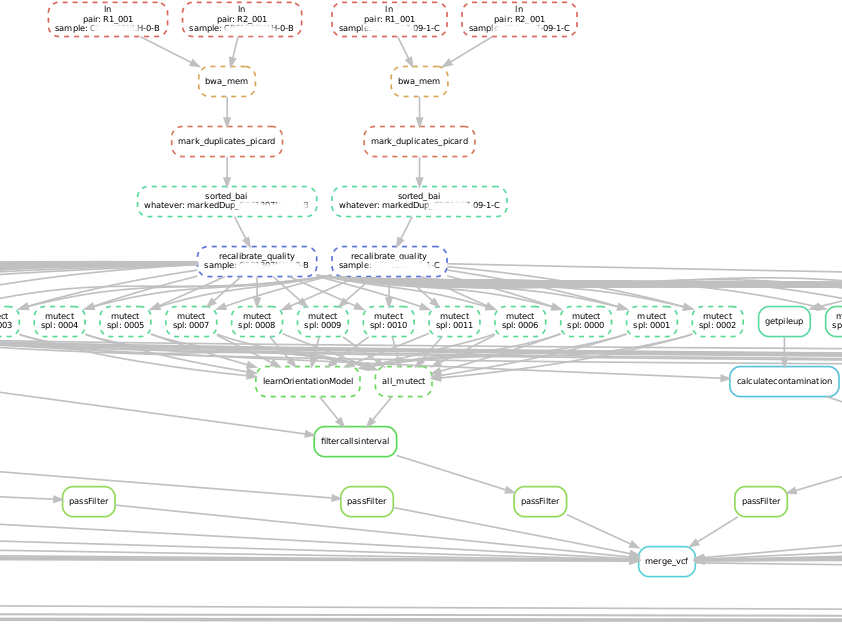
\includegraphics[width=1\textwidth]{./img/dag.png}\end{figure}
\end{frame}

\begin{frame}
\frametitle{Let's count the number of reads in fastq files!}
Example Snakefile on moodle. \\

\texttt{snakemake -p} prints the commands it executes, \texttt{-n} is a dry-run (does not run anything but shows what it would do).
\\
\texttt{-f} forces it to re-run a rule even if its output is already there.
\end{frame}

\begin{frame}[fragile]
\frametitle{Our first real rule}
\begin{python}
rule count_reads:
	input: "fastq/a.fastq.gz"
	output: "a_n_reads.txt"
	run: 
		n_rows = 0
		with gzip.open(input.fq, "rb") as fq:
		    for line in fq:
		        n_rows = n_rows + 1
		with open(output.n, "w") as of:
		    of.write("{}\n".format(n_rows/4))

\end{python}
But we have more than one sample!
\end{frame}

\subsection{Wildcards}

\begin{frame}[fragile]
\frametitle{DRY: Don't repeat yourself...be lazy!}

\texttt{\{n\}} creates a wildcard called \emph{n}, it can be used in input/output/params - all the wildcards that you use in input should also be in output. \\
\vspace{0.5cm}

Inside the rules you can refer to them with \texttt{wildcards.n}
\begin{lstlisting}[basicstyle=\tiny]
rule count_reads:
    input: fq="fastq/{sample}.fastq.gz"
    output: n="{sample}_n_reads.txt"
    run: 
        n_rows = 0
        with gzip.open(input.fq, "rb") as fq:
            for line in fq:
                n_rows = n_rows + 1
        with open(output.n, "w") as of:
            of.write("{}\n".format(n_rows/4))
\end{lstlisting}

\begin{tiny}
Let's go and add this to our makefile!
\end{tiny}
\end{frame}

\begin{frame}[fragile]
\frametitle{How can we ask many files at once?}
\begin{python}[basicstyle=\small]
SAMPLES = ['a', 'b', 'c', 'd']
rule all_n_reads:
   input: expand("{sample}_n_reads.txt", sample=SAMPLES)
\end{python}
We can set up a rule without any output that will have as input all the results of the 'last' step of our pipeline - i.e. all the results of \texttt{count\_reads}. \\
We'll then be able to invoke it via its name: \texttt{\$ snakemake all\_n\_reads}. The rule itself won't do anything but when we will launch it,
it will trigger the execution of all ``previous'' rules in the pipeline.
\end{frame}


\begin{frame}[fragile]
\frametitle{How can we ask many files at once? - II}
\texttt{expand()} is used to populate filenames putting values from vectors where wildcards are: \\
\begin{python}[basicstyle=\small]
SAMPLES = ['a', 'b', 'c', 'd']
rule all_counts:
   input: expand("{sample}_n_reads.txt", sample=SAMPLES)
\end{python}
will result in the same as:
\begin{python}[basicstyle=\small]
rule all_counts:
   input: 'a_n_reads.txt', 'b_n_reads.txt', 
   	  'c_n_reads.txt', 'd_n_reads.txt'
\end{python}
\tiny{
But, at this point you know, we are lazy and want to put only once in a variable the list of samples and refer to it everywhere else, in this way our 'rules' will be
\textcolor{galon}{general} and we will define only some \textcolor{novak}{project-specific variables} (i.e. names of samples) once. Moreover SAMPLES too can be
populated with code \ldots
}
\end{frame}

\begin{frame}[fragile]
\frametitle{Summarizing rules}
Our ``all'' rules can sometimes be empty as we discussed before, but
after having aligned many samples and obtained their reads counts on genes it's often useful to put all the counts in a single file, or put together
the info about the number of aligned reads.
\begin{python}[basicstyle=\small]
rule all_counts:
   input: expand("{sample}_n_reads.txt", sample=SAMPLES)
   output: "all_n_reads.txt"
   shell: "cat {input} > {output}"
\end{python}
\end{frame}

\subsection{Details}
\begin{frame}[fragile]
\frametitle{Accessing input/output from R script directives}
\begin{tiny}
snakemake creates an object for us inside our R scripts called from rules: snakemake. It is a S4 object
with slots that are directives, storing lists of our input/output:
\end{tiny}
\begin{python}
rule example:
	input: infile1="file1.tsv", infile2="file2.tsv"
	output: plot="plot.png"
	script: "niceplot.R"
	
# In niceplot.R:
snakemake@input[['infile1']] # will be storing 'file1.tsv'
snakemake@input[['infile2']] # will be storing 'file2.tsv'
snakemake@output[['plot']]  # will be storing 'plot.png'
\end{python}
\begin{tiny}
Better to use names for input/output directives when you call R/have more than one!
\end{tiny}
\end{frame}

\begin{frame}[fragile]
\frametitle{Let's represent graphically our n. of reads}
\begin{columns}
\column{.5\textwidth}
%\begin{tiny}
\begin{lstlisting}[basicstyle=\tiny]
rule plot:
    input: n="all_n_reads.txt"
    output: plot="n_reads.png"
    script: "histogram_reads.R"
\end{lstlisting}
%\end{tiny}
\column{.5\textwidth}
\begin{figure}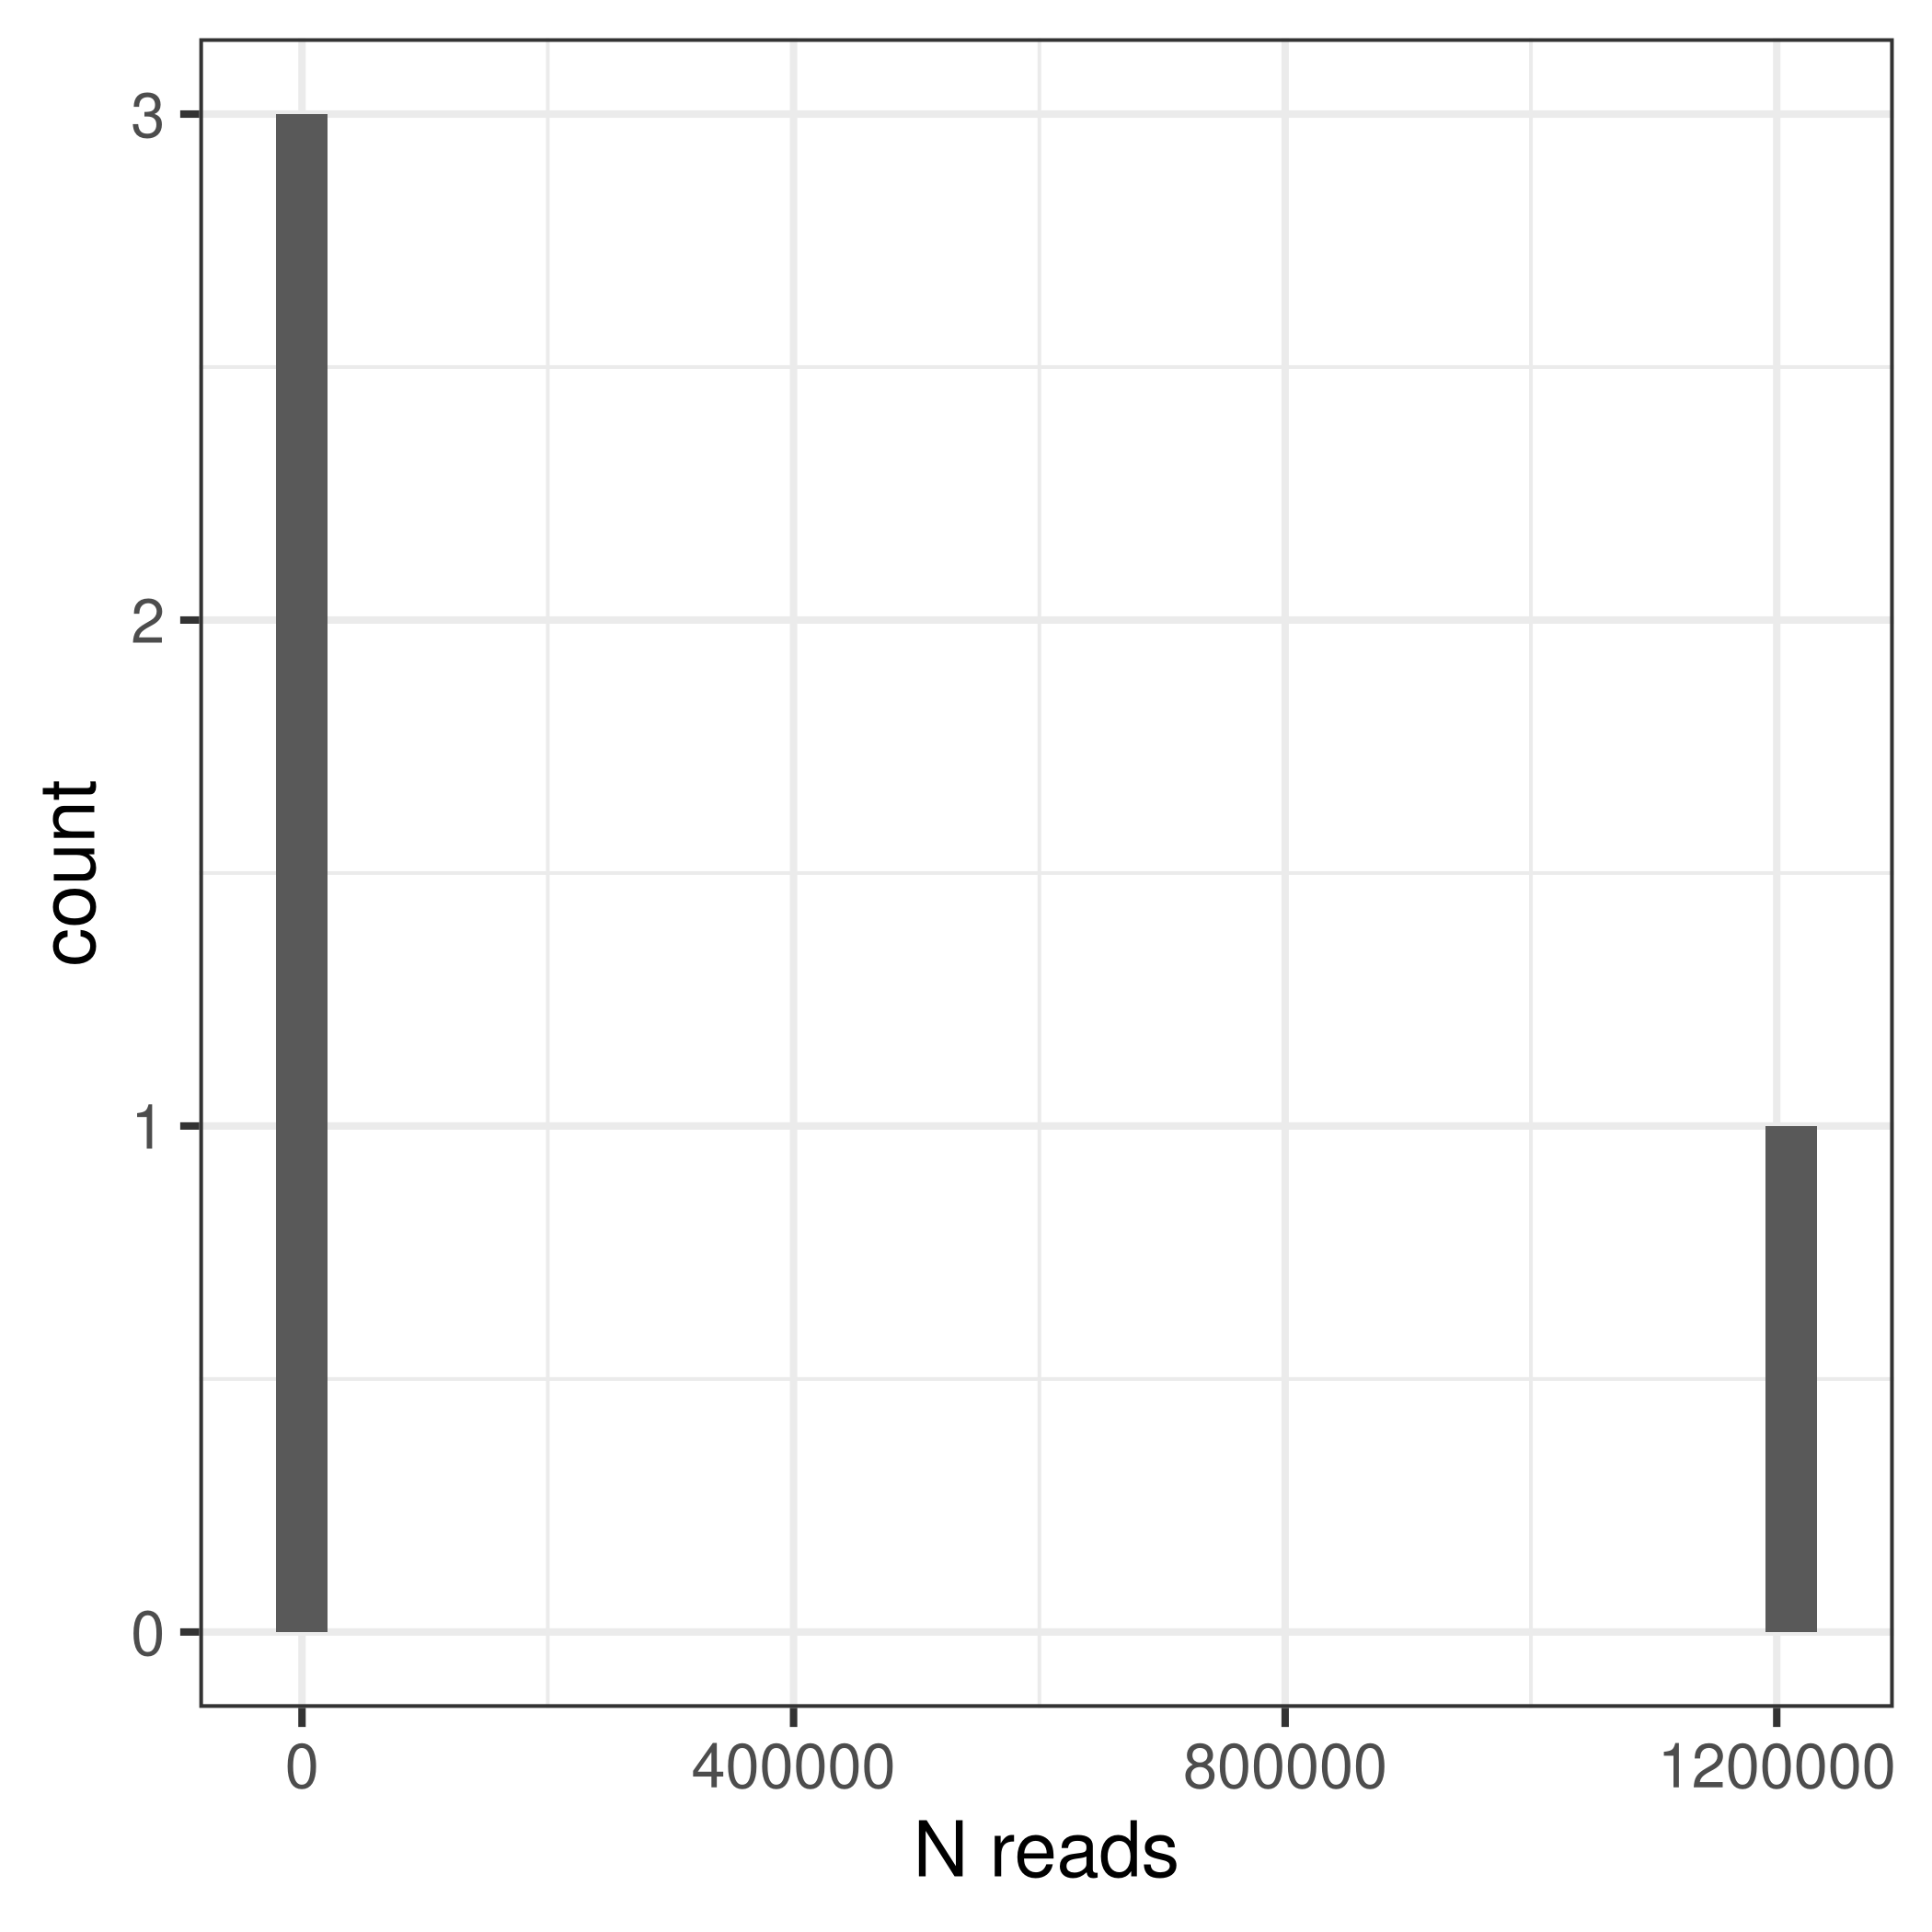
\includegraphics[width=0.95\textwidth]{./img/n_reads.png}\end{figure}
\end{columns}
\end{frame}


\subsection{More details}
\begin{frame}[fragile]
\frametitle{The params directive}
\begin{footnotesize}
We often pass arguments to a command, if we do not need to \emph{include} them in our input/output chain via wildcards we can include them in the params directive, to avoid
\textcolor{beer}{hardcoding} them in the rules themselves. If we obtain them from variables that we define in a specific position in our Snakefile we will be able to rapidly change them: think about
moving an example pipeline on your laptop to a big server. It's reasonable to expect to have several rules that uses the 'number of threads', and we do not want to change all of them.
\end{footnotesize}

\begin{columns}
\column{.5\textwidth}
\begin{beamerboxesrounded}[upper=upper_box,lower=lower_box,shadow=true]{Don't do this}
\begin{lstlisting}[basicstyle=\tiny]
rule get_counts:
   ...
   shell: 
   """
   featureCounts -t 1
   """
\end{lstlisting}
\end{beamerboxesrounded}

\column{.5\textwidth}
\begin{beamerboxesrounded}[upper=upper_box2,lower=lower_box,shadow=true]{But this}
\begin{lstlisting}[basicstyle=\tiny]
THREADS=1
rule get_counts:
   ...
   params: threads=THREADS
   shell: 
   """
   featureCounts -t {params.threads}
   """
\end{lstlisting}
\end{beamerboxesrounded}
\end{columns}
\end{frame}

\begin{frame}[fragile]
\frametitle{Wildcards are not only for list of samples \ldots}

Let's suppose you want to try different \textcolor{beer}{alignment parameters} and evaluate the resulting \% of aligned reads. \\
You can have the same input for a rule and use a wildcard as output to determine one parameter of your tool:
\begin{python}[basicstyle=\tiny]
rule align:
   input: "{sample}.fastq.gz"
   output: "{sample}_align{multimap}.bam"
   shell: " ... {wildcards.multimap} ...  {input} ..."
\end{python}

\end{frame}


\begin{frame}
\frametitle{We can put code everywhere to fine-tune our pipeline}
What if we have a paired end sequencing?

We should be able to count n. of reads in \textcolor{beer}{files with different names}:
\texttt{\{sample\}.fastq.gz} or \texttt{\{sample\}.R1.fastq.gz} - since R2 will have the same
number of reads we can access only R1, but let's suppose that given a sample we want to use the R1 file
if it exists and the single-end file otherwise (this is a risky logic in the real world, probably \ldots as an 
exercise try to modify our example code to print an error if a samples has both the R1 and the unpaired ends file!).

\end{frame}


\begin{frame}[fragile]
\begin{lstlisting}[basicstyle=\tiny]
def find_R1_or_other(wildcards):
    import os
    if os.path.isfile(os.path.join('fastq', wildcards.sample+'.R1.fastq.gz')):
        return(os.path.join('fastq', wildcards.sample+'.R1.fastq.gz'))
    else:
        return(os.path.join('fastq', wildcards.sample+'.fastq.gz'))

rule count_reads_R1_precedence:
    input: fq=find_R1_or_other
    output: n="{sample}_nn_reads.txt"
    run: 
        n_rows = 0
        with gzip.open(input.fq, "rb") as fq:
            for line in fq:
                n_rows = n_rows + 1
        with open(output.n, "w") as of:
            of.write("{}\n".format(n_rows/4))
\end{lstlisting}
\end{frame}


\begin{frame}
\frametitle{Take home message}
Snakemake is a workflow management system that makes bioinformaticians lifes easier, basically allowing them
to define their \textcolor{galon}{pipelines} once and then running them for lots of different datasets and on different
computational resources with minimal effort. \\
Its behaviour is defined by \textcolor{novak}{rules}, whose order is defined by a chain of input-output, and whose actions
can be defined with shell commands, various scripts (such as R) or python code. With little python knowledge pipelines can be tailored
at (almost) every level.
\\ The price we need to pay is to learn it and think about how we want to structure
the pipeline instead than dive in launching commands by hand (this will still be needed to determine how to write single rules!).
\end{frame}

\begin{frame}
\frametitle{Material}
These slides show all the Snakemake aspects that are relevant for this course. \\ If you want some reference material I suggest
you to start here: \url{https://snakemake.readthedocs.io/en/stable/tutorial/basics.html}
\end{frame}
% -j as a first scalability asset

\end{document}
